In section~\ref{introOverview}, six core components of this project were identified. The first
two, ODE solving and rigid body dynamics, were introduced in the last chapter. In this chapter
I shall leave the solid ground of textbook material and delve into some less well-known methods.
I have already discussed how to formulate constraints, so we can now put together constraints
and rigid bodies to create articulated bodies in section~\ref{articulatedBodies}. Then I will
explore how to detect and handle collisions and contacts between bodies in
sections~\ref{collisionDetection} and~\ref{collisionHandling}. Finally, in
section~\ref{implementation} I will show how all the theory was cast into code to form a
working simulation, and which challenges I faced along the way.


\section{Articulated bodies\label{articulatedBodies}}

\subsection{Modelling the human body}

The human body's selection of joint types is quite limited compared to the range of connectors
found in machines~\cite{Kalra:95}: for example, there are no sliding joints or screws. The simple
types of joint found in human bodies are ball-and-socket joints allowing rotation about three axes
(like shoulders and hips), and revolute joints limited to a single axis (like knees and elbows).
The issue is made more complicated by compound joints like the spine, and motion which occurs
along the length of a limb rather than at a joint (like rotating the wrist about the axis of
the lower arm, which occurs through a relative shift of the ulna and radius
bones~\cite{Anatomy:03}).

To make the model manageable, I shall choose to be anatomically ignorant and assume that two
adjacent limbs are connected by a single joint, and that rotation occurs only about this joint.
Each bone has a local coordinate system whose origin lies at the joint to the parent bone.
This is illustrated in figure~\ref{jointsFigure}.

\begin{figure}
\centerline{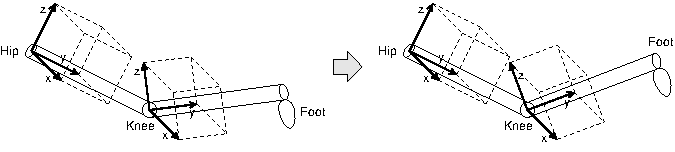
\includegraphics{figures/joint1}}
\caption{Two bones connected by a revolute joint, e.g.\ a knee. Rotation is constrained to be
    possible only about the local x~axis of the knee, but not the local y~axis
    (the lower leg itself) or the local z~axis (sideways).\label{jointsFigure}}
\end{figure}

There are different ways of formulating this model, but I choose to assume initially that every
joint is a ball-and-socket type. If it is not, additional constraints are added to restrict
the permitted axes of rotation.

\subsection{Ball-and-socket joints}

The position of a joint is a particular offset from the centre of mass in one body's frame, and a
different offset from the other body's centre of mass. While the bodies may move around, these
offsets stay constant (as seen in the body's frame).

Figure~\ref{ballAndSocketFigure} gives an example: here, the configuration of bodies satisfies the
ball-and-socket constraint iff $\ve{a}+\ve{s} = \ve{b}+\ve{t}$, i.e.\ if the joint has not
separated. We can rewrite this to give the constraint function
\begin{equation}
\ve{c} = \ve{a} + \ve{s} - \ve{b} - \ve{t}
\end{equation}
which equals \ve{0}, the three-dimensional null vector, iff the constraint is satisfied.

\begin{figure}
\psfrag{frag:o}{\ve{O}}
\psfrag{frag:a}{\ve{a}}
\psfrag{frag:b}{\ve{b}}
\psfrag{frag:s}{\ve{s}}
\psfrag{frag:t}{\ve{t}}
\centerline{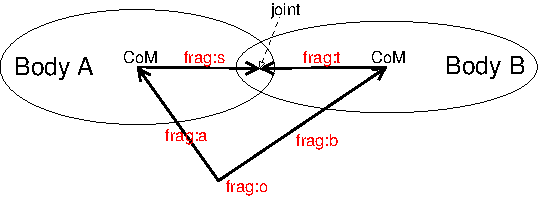
\includegraphics{figures/joint2}}
\caption[]{A valid ball-and-socket joint configuration. \ve{s} is constant in body~A's frame,
    while \ve{t} is constant in the frame of body~B. In the world frame, these two vectors
    therefore rotate according to their respective body's orientation.\label{ballAndSocketFigure}}
\end{figure}

\subsection{Rotation constraints}

In the case of an elbow or a knee, we also need to prohibit the rotation about particular axes.
After some thought I came up with the constraint function
\begin{equation}
c = \Re(\tilde{\ve{n}}\q{p}^{-1}\q{q})
\end{equation}
in which \q{p} is the quaternion of orientation for body~A, \q{q} the quaternion for body~B, and
\ve{n} a vector pointing along the prohibited axis in body~A's frame. Setting $c$ to zero ensures
that no rotation occurs about the axis~\ve{n}. If two different axes are prohibited with two
separate constraints, then rotation is only possible about a single axis orthogonal to the two
prohibited axes. Further details on this constraint are given in appendix~\ref{constrJoystick}.

\subsection{Angle limitation}

The constraints described so far capture most of the features of the human skeleton, with one
exception: if rotation is permitted about some axis, there is no limit to the amount of rotation
that can occur. For example, permitting Alfred to look left and right would allow the simulation
to rotate his head by an arbitrary amount~-- quite literally to screw his head off. Imposing
limits on the angle of rotation as well as the axis is possible but more complicated, and will
be explained in section~\ref{generalizedCollisions}. It may be worth noting that this is our
first example of a non-holonomic constraint, and thus lies beyond the capabilities of Lagrangian
mechanics.
